\documentclass[12pt]{article}
\usepackage[spanish]{babel}
\usepackage{amsmath}
\usepackage{amsfonts}
\usepackage{graphicx}
\usepackage{ragged2e}
\graphicspath{ {images/} }
\usepackage{fancyvrb}
\usepackage{enumitem}
\usepackage[utf8x]{inputenc} 
\begin{document}

\title{\textbf{Basic Modeling for Discrete Optimization}}
\date{}
\maketitle

\textit{Apuntes del curso de Coursera: Basic Modeling for Discrete Optimization, en español. Por: Juan Marcos Caicedo M. @ Universidad del Valle, Cali, Colombia}

\vspace{1cm}

\textbf{1.1.1 Primeros pasos (First Steps)}

\begin{justify}
Los hermanos Guan Yu, Liu Bei, y Zhang Fei van a reclutar un ejército para vencer al Ejército  de los Turbantes Amarillos. Tienen disponibilidad para contratar guereros de 4 distintas aldeas: Feng, Liu, Zhao y Jian. Cada guerrero de cada aldea tiene una fuerza, un costo, y se tiene un límite de cuantos soldados de cada aldea pueden tomar:
\end{justify}

\begin{table}[h]
\begin{tabular}{|l|l|l|l|l|}
\hline
       & Feng & Liu & Zhao & Jian \\ \hline
Fuerza & 6    & 10  & 8    & 40   \\ \hline
Costo  & 13   & 21  & 17   & 100  \\ \hline
Límite & 1000 & 400 & 500  & 150  \\ \hline
\end{tabular}
\end{table}

\begin{justify}
Tenemos, entonces, para resolver este problema, algunas \textbf{restricciones}:
\end{justify}

\begin{itemize}
\item El presupuesto que los hermanos poseen, que es de 10000.
\item La cantidad máxima de soldados que podemos tomar de cada aldea.
\end{itemize}

\begin{justify}
Y poseemos un \textbf{objetivo}:
\end{justify}

\begin{itemize}
\item Maximizar la fuerza total de nuestro ejército.
\end{itemize}

\begin{justify}
Guan Yu, sugiere contratar los mejores y más caros soldados: 100 soldados de la aldea Jian, para un total de 4000 de fuerza.
\end{justify}

\begin{justify}
Zhang Fei, sugiere contratar el la mayor cantidad de los soldados baratos: 769 soldados de la aldea Feng, que nos da un total de 4614.
\end{justify}

\begin{justify}
En este punto nos preguntamos: \textbf{¿Podemos dar una mejor respuesta? ¿Podemos hacerlo mejor?}. Podemos expresar esto como un modelo matemático:
\end{justify}

\begin{justify}
Maximizar $6F + 10L + 8Z + 40J$ sujeto a:
\end{justify}

\begin{itemize}
\item $13F + 21L + 17Z + 100J \leq \text{presupuesto}$
\item $0 \leq F \leq 1000$
\item $0 \leq L \leq 400$
\item $0 \leq Z \leq 500$
\item $0 \leq J \leq 150$
\item $F, L, Z, J \in \mathbb{Z}, \text{presupuesto} = 10000$
\end{itemize}

\begin{justify}
Y para ello podemos escribri un modelo en \textbf{MiniZinc} que resuelve esto:
\end{justify}

\begin{Verbatim}
int: budget = 10000;
var 0..1000: F;
var 0..400: L;
var 0..500: Z;
var 0..150: J;

constraint 13*F + 21*L + 17*Z + 100*J <= budget;

solve maximize 6*F + 10*L + 8*Z + 40*J;

output ["F = \(F), L = \(L), Z = \(Z), J = \(J)"];

\end{Verbatim}

\begin{justify}
Detallando el modelo:
\end{justify}

\begin{itemize}
\item En la primera línea, tenemos una \textbf{definición de parámetros}. Definimos un nuevo parámetro "budget" (presupuesto) que toma el valor de 10000. El modelo, donde vea la palabra budget, verá el valor de 10000. 
\item Entre las líneas 2 y 5 hay declaraciones de \textbf{variables de decisión}. Son 4 decisiones que se hacen: ¿Cuántos soldados contratamos de cada una de las 4 aldeas?. Son variables enteras, en las que escogemos un rango en los cuales toman valores. Esto es donde los 3 heroes deben decidir.
\item En la línea 6 hay una \textbf{restricción}, que está forzando a que solo contratemos el numero de soldados que podemos adquirir con el presupuesto disponible.
\item En la línea 7 tenemos la \textbf{función objetivo}, debemos maximizar la fuerza de nuestro ejército y así se representa de manera matemática.
\item En la última línea tenemos una expresión de salida (output), y es lo que se imprime cuando encontramos una solución, e imprime el valor de cada variable de decisión. 
\end{itemize}

\begin{justify}
\textbf{Variables en MiniZinc: MiniZinc tiene dos tipos de variables: parámetros y variables de decisión:}
\end{justify}

\begin{itemize}
\item Parámetros: Son como las variables en un lenguaje de programación estándar. Deben ser asignadas a un valor (pero sólo una vez). Se declaran con un tipo: int, float o bool. Es un objeto matemático y su valor es inmutable. Por ejemplo, el presupuesto es de 10000, no puede tener después un valor de 18000. Sólo puede tomar un valor. (Puede llevar la palabra reservada par). Ejemplos:
\begin{Verbatim}
int: i = 3;
par int: i = 3;
int: i; i = 3;
\end{Verbatim}
\item Variables de decisión: Son como variables en matemáticas. Se declaran con la palabra reservada var. Estas son las variables que el solver trabajará con sus valores y probará. Son asignadas solo una vez con una expresión fija. Poseen un rango escrito: l..u (secuencia continua de enteros de l a u). Ejemplos (expresiones lógicamente equivalentes):
\begin{Verbatim}
var int: i; constraint i >= 0; constraint i <= 4;
var 0..4: i;
var {0,1,2,3,4}: i;
\end{Verbatim}
También:
\begin{Verbatim}
var int: i = x + 3;
var int: i; constraint i = x + 3;
\end{Verbatim}
\end{itemize}

\begin{justify}
\textbf{Restricciones en MiniZinc:} Restricciones con aritmética básica sonc readas usando los operadores relaciones aritméticos estándar: \begin{verbatim}
=, !=, >, <, >=, <=
\end{verbatim}
Se escriben con la palabra reservada constraint:
\end{justify}
\begin{Verbatim}
constraint x + y <= 10
\end{Verbatim}

\begin{justify}
\textbf{Salidas (output) en MiniZinc:} Tienen la forma:
\end{justify}
\begin{Verbatim}
output <list of strings>;
\end{Verbatim}

\begin{justify}
Y los literales string (string literals) son como en C: encerrados entre comillas dobles. Existen funciones como \begin{Verbatim}
\n y \t -> salto de linea y tab
show(v) -> el valor de v como string
\(v) -> muestra a v dentro de un literal de string
"casa"++"bote" -> concatenación de strings
\end{Verbatim} 
\end{justify}

\begin{justify}
\textbf{Correr modelo en MiniZinc:} Nuestro modelo army.mzn:
\end{justify}

\begin{Verbatim}
int: budget = 10000;
var 0..1000: F;
var 0..400: L;
var 0..500: Z;
var 0..150: J;

constraint 13*F + 21*L + 17*Z + 100*J <= budget;

solve maximize 6*F + 10*L + 8*Z + 40*J;

output ["F = \(F), L = \(L), Z = \(Z), J = \(J)"];

\end{Verbatim}

\begin{justify}
Se puede correr en la terminal usando:
\end{justify}

\begin{Verbatim}
$ minizinc army.mzn
\end{Verbatim}

\begin{justify}
Dará la siguiente salida:
\end{justify}

\begin{Verbatim}
F = 0, L = 392, Z = 104, J = 0
----------
==========
\end{Verbatim}

\begin{justify}
La fuerza total es 4752 y el tamaño es 496. Que es mejor que las propuestas de los otros héroes.
\end{justify}

\begin{justify}
La línea ---------- significa que halló una solución.
\end{justify}

\begin{justify}
La línea ========== significa que halló \textbf{la mejor solución posible}.
\end{justify}

\begin{justify}
Modelos (archivos) de MiniZinc deben terminar en .mzn
\end{justify}

\begin{justify}
El modelo también se puede correr con el botón \textit{Run} del IDE.
\end{justify}

\newpage

\textbf{1.1.2 Segundo Modelo (Second Model)}

\begin{justify}
Después de la contratación de los soldados, empezaron el entrenamiento. Sin embargo, algunos soldados huyeron pues el entrenamiento era muy duro. Los 3 hermanos desean saber cuantos soldados les quedaron sin contarlos uno a uno. Hicieron lo siguiente:
\end{justify}

\begin{itemize}
\item Organizaron a los soldados en 5 líneas de igual tamaño y sobraron 2 soldados.
\item Organizaron a los soldados en 7 líneas de igual tamaño y sobraron 2 soldados.
\item Organizaron a los soldados en 12 líneas de igual tamaño y sobró 1 soldado.
\end{itemize}

\begin{justify}
Podríamos resolverlo usando el siguiente modelo de MiniZinc (count.mzn):
\end{justify}

\begin{Verbatim}
var 100..800: army;

constraint army mod 5 = 2;
constraint army mod 7 = 2;
constraint army mod 12 = 1;

solve satisfy;
\end{Verbatim}

\begin{justify}
En este caso no estamos tratando de optimizar algo en concreto, solo estamos tratando de encontrar una solución. Hay alguna solución a este problema?. Este es no es un \textbf{problema de optimización discreta}, es un \textbf{problema de satisfacción discreta}. También nótese que no hay output. El resultado de la ejecución en terminal del modelo es:
\end{justify}

\begin{Verbatim}
army = 457;
----------
\end{Verbatim}

\begin{justify}
La falta de una línea ========== indica que pueden haber otras soluciones. Si corremos:
\end{justify}

\begin{Verbatim}
$ minizinc --all-solutions count.mzn
\end{Verbatim}

\begin{justify}
Obtenemos:
\end{justify}

\begin{Verbatim}
army = 457;
----------
==========
\end{Verbatim}

\begin{justify}
Lo cuál indica que no hay otras soluciones. \textbf{Tienen que haber} 457 soldados restantes. Se puede configurar en el IDE que de todas las soluciones (predeterminado para problemas de optimización). Para problemas de satisfacción, no es predeterminado mostrar todas las soluciones. Como se había visto, el modelo no tiene output.
\end{justify}

\begin{justify}
Sin embargo, MiniZinc, por defecto manda como output todas las variables declaradas que no están asignadas a una expresión.
\end{justify}

\begin{justify}
En los problemas de satisfacción, no es necesario buscar una solución óptima. 
\end{justify}

\begin{justify}
Dentro de las \textbf{Restricciones} no sólamente hay igualdades o desigualdades lineales: también puede haber modulo, multiplicaciones, divisiones, distinto de ($\neq$), y restricciones mucho más complejas.
\end{justify}

\newpage

\textbf{1.1.3 Tercer Modelo (Third Model)}

\begin{justify}
Liu Bei, Guan Yu, y Zhang Fei deseaban que un hombre ostentoso les prestara caballos para la guerra. El hombre de los caballos se preguntó si los hermanos realmente eran talentosos para hacer buen uso de sus caballos. Les dió un problema y les prometió que les prestaría los caballos si resuelven dicho problema.
\end{justify}

\begin{center}
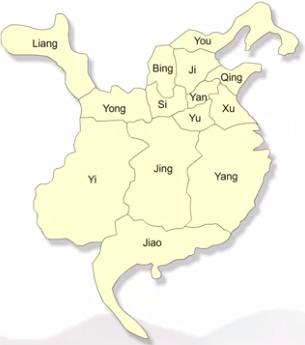
\includegraphics[scale=0.5]{han}
\end{center}

\begin{justify}
Les dió un mapa de la Dinastía Han, y debían colorar el mapa usando como máximo 4 colores, tal que las provincias adyacentes no compartieran el mismo color. Miremos cómo resolver este problema con un modelo de MiniZinc (color.mzn):
\end{justify}

\begin{Verbatim}
enum COLOR = {GREEN, BLUE, PINK, YELLOW};

var COLOR: Si;
var COLOR: Yan;
var COLOR: Yu;
var COLOR: Xu;
var COLOR: Qing;
var COLOR: Ji;
var COLOR: You;
var COLOR: Bing;
var COLOR: Yong;
var COLOR: Liang; 
var COLOR: Yi;
var COLOR: Jing;
var COLOR: Yang;
var COLOR: Jiao;

constraint Liang != Yong;
constraint Yong != Yi;
constraint Yong != Jing;
constraint Yong != Si;
constraint Yi != Jing;
constraint Yi != Jiao;
constraint Jiao != Jing;
constraint Jiao != Yang;
constraint Jing != Yang;
constraint Jing != Yong;
constraint Jing != Si;
constraint Jing != Yu;
constraint Yang != Yu;
constraint Yang != Xu;
constraint Yu != Si;
constraint Yu != Yan;
constraint Yu != Xu;
constraint Xu != Yan;
constraint Xu != Qing;
constraint Yan != Si;
constraint Yan != Ji;
constraint Yan != Ji;
constraint Yan != Qing;
constraint Qing != Ji;
constraint Ji != You;
constraint Ji != Bing;
constraint Ji != Si;
constraint You != Bing;
constraint Bing != Si;

solve satisfy;
\end{Verbatim}

\begin{justify}
En el modelo se tiene un \textbf{tipo enumerado (enumerated type)} llamado COLOR, que es hecho a partir de 4 colores: verde, azul, rosado y amarillo. Cada una de las provincias es declarada como una variable de este tipo enumerado, COLOR. Por otro lado, tenemos las restricciones que nos permiten decir que cada provincia vecina con la otra sean de distinto color. Podemos correr el modelo usando:
\end{justify}

\begin{Verbatim}
$ minizinc color.mzn
\end{Verbatim}

Obtenemos:

\begin{Verbatim}
Si = BLUE;
Yan = GREEN;
Yu = PINK;
Xu = YELLOW;
Qing = BLUE;
Ji = PINK;
You = BLUE;
Bing = GREEN;
Yong = PINK;
Liang = GREEN;
Yi = BLUE;
Jing = GREEN;
Yang = BLUE;
Jiao = PINK;
----------
\end{Verbatim}

\begin{justify}
Que es, por supuesto, una solución a ese problema. Nóteseque no teniamos función output, entonces arrojó todas las variables de decisión con valores posibles que cumplen las restricciones impuestas.
\end{justify}

\begin{justify}
En este ejemplo se ve una característica nueva de MiniZinc: enumareted types (tipos enumerados), son una manera de definir un conjunto finito de objetos que poseen nombre.
\end{justify}

\begin{itemize}
\item Podemos entonces hacer que variables de decisión y parametros sean tipos enumerados. 
\item Los índices del array pueden ser tipos enumerados.
\item También, conjuntos pueden ser tipose enumerados.
\end{itemize}

\begin{justify}
Los tipos enumerados son declarados con la palabra clave \textit{enum}, de la siguiente manera: \textit{enum} enum-name. Donde enum-name = \{ id1, ..., idn\}. Podemos declarar variables que tomarán valores de tipos enumerados (como se vio en el ejemplo): var enum-name: var-name.
\end{justify}

\begin{justify}
Si modificamos el modelo anterior, los colores reduciendolos solo a 3:
\end{justify}

\begin{Verbatim}
enum COLOR = {GREEN, BLUE, PINK};
\end{Verbatim}

\begin{justify}
Corriendolo obtenemos:
\end{justify}


\begin{Verbatim}
=====UNSATISFIABLE=====
\end{Verbatim}

\begin{justify}
Esto significa que no hay solución alguna al problema, con 3 colores.
\end{justify}

\begin{justify}
\textbf{Resumen:} Tipos enumerados:
\end{justify}

\begin{itemize}
\item Introducen un conjunto de objetos nombrados
\item Util para tener <<seguridad de tipos (type safety)>> en los modelos
\item Se verá más de tipos enumerados (enumerated types)
\end{itemize}

\begin{justify}
Existen modelos \textbf{insatisfactibles}. Debemos tener en cuenta que no todo modelo tiene solución.
\end{justify}

\begin{justify}
También resolvimos un problema de coloreado de grafos (graph coloring problem), que es un problema clásico en la teoría de grafos, y tiene aplicaciones como registro de asignaciones, horarios, etc. Coloreado de grafos puro es manejado mejor por algoritmos especializados.
\end{justify}

\newpage

\textbf{1.1.4 Modelos e Instancias (Models and Instances)}

\begin{justify}
Nuestros tres héroes están interesados en conocer: Si hubiesen tenido más dinero, qué tan mejor ejército hubieran conseguido con respecto a su actual? A continuación, el modelo del Ejército que hicimos en lecciones pasadas, pero con un pequeño cambio: ya no especificamos que el presupuesto es 10000, lo dejamos sin especificar (armyd.mzn).
\end{justify}

\begin{Verbatim}
int: budget;
var 0..1000: F;
var 0..400: L;
var 0..500: Z;
var 0..150: J;

constraint 13*F + 21*L + 17*Z + 100*J <= budget;

solve maximize 6*F + 10*L + 8*Z + 40*J;

output ["F = \(F), L = \(L), Z = \(Z), J = \(J)"];
\end{Verbatim}

\begin{justify}
Cuando vayamos a correr el modelo, debemos darle ese parámetro de algún lado, puesto que no es una decisión, debe tener un valor asignado.. Entonces, podríamos correr nuestro modelo, añadiendole un archivo de datos (data file), llamado army.dzn:
\end{justify}

\begin{Verbatim}
$ minizinc armyd.mzn army.dzn
\end{Verbatim}

\begin{justify}
Y el contenido de army.dzn es:
\end{justify}

\begin{Verbatim}
budget = 20000;
\end{Verbatim}

\begin{justify}
La ejecución resulta en:
\end{justify}

\begin{Verbatim}
F = 243, L = 398, Z = 499, J = 0
----------
==========
\end{Verbatim}

\begin{justify}
Que sería el mejor ejército con el nuevo presupuesto de 20000.
\end{justify}

\begin{justify}
También podemos, si deseamos, poner el archivo de datos directamente en la terminal de la manera:
\end{justify}

\begin{Verbatim}
$ minizinc armyd.mzn -D"budget = 20000;"
\end{Verbatim}

\begin{justify}
También se puede usar el IDE para proveer estos datos no especificados, al correr el modelo en \textit{Run}, el IDE abrirá una ventana donde se debe ingresar los valores de parámetro faltantes.
\end{justify}

\begin{justify}
Otra manera, es si se tiene cargado el archivo army.dzn, se puede seleccionar un archivo de datos (data file).
\end{justify}

\begin{justify}
Los 3 hermanos observaron que tenían pocos soldados, entonces planearon reclutar más, pero para ello necesitarían un préstamo de dinero de algún hombre de negocios para poder conseguir más soldados. Consiguieron un hombre de negocios que les ayudaría con el préstamo.
\end{justify}

\begin{justify}
El hombre de negocios accedió a prestarles el dinero, pero con la condición de que devolverían el préstamo sumado a unos intereses, durante 4 pagos realizados en el siguiente año. Cada pago se haría en cada estación (primavera, verano, otoño, invierno). Liu Bei quiere averiguar cuanto tienen que pagar exactamente en cada estación. 
\end{justify}

\begin{justify}
Cómo funcionará el préstamo:
\end{justify}

\begin{itemize}
\item El prestamista otoga como préstamo una cantidad $P$, es un capital que es el saldo inicial.
\item Cada cuarto de año, estación, cuatrimestre, se requiere dar un reembolso $R$.
\item La tasa de interés $I$ en cada cuarto de año.
\item Al final del i-ésimo cuarto el saldo adeudado $B_{i}$ está dado por:
\begin{itemize}
\item El saldo anterior
\item Más el interés sobre el saldo anterior
\item Menos el reembolso
\end{itemize}
\end{itemize}

\begin{justify}
Un modelo en MiniZinc sobre esto:
\end{justify}

\begin{Verbatim}
% variables
var float: R;  % quarterly repayment
var float: P;  % principal initially borrowed
var 0.0 .. 2.0: I;  % interest rate

% intermediate variables
var float: B1; % balance after one quarter
var float: B2; % balance after two quarters
var float: B3; % balance after three quarters
var float: B4; % balance owing at end

constraint B1 = P * (1.0 + I) - R;
constraint B2 = B1 * (1.0 + I) - R;
constraint B3 = B2 * (1.0 + I) - R; 
constraint B4 = B3 * (1.0 + I) - R;

solve satisfy;

output [
 "Borrowing ", show_float(0, 2, P), " at ", show_float(0,2,I*100.0), 
 "% interest, and repaying ", show_float(0, 2, R), 
  "\nper quarter for 1 year leaves ", show_float(0, 2, B4), " owing\n"
];
\end{Verbatim}

\begin{justify}
Tenemos nuevas características:
\end{justify}

\begin{itemize}
\item Variables flotantes como R, P, I, B1, B2, B3 y B4.
\item Variables como R, P desconocidas inicialmente (y sin rango)
\item Un rango flotante en I: 0.0..2.0, interés entre 0 y 200%
\end{itemize}

\begin{justify}
Ahora, hagamonos unas cuantas preguntas sobre este modelo:
\end{justify}

\begin{justify}
\textbf{Primera Instancia:}Liu Bei quiere recibir como préstamo \$10000 con tasa de interés del 4\%, reembolsando \$2600. Cuánto debe al final?
\end{justify}

\begin{justify}
Podemos crear un archivo de datos, loan1.dzn, que contenga:
\end{justify}

\begin{Verbatim}
I = 0.04;
P = 10000.0;
R = 2600.0;
\end{Verbatim}

\begin{justify}
Corriendo el modelo con el archivo de datos:
\end{justify}

\begin{Verbatim}
$ minizinc loan.mzn loan1.dzn
\end{Verbatim}

\begin{justify}
Obtenemos:
\end{justify}

\begin{Verbatim}
Borrowing 10000.00 at 4.00% interest, and repaying 2600.00
per quarter for 1 year leaves 657.78 owing
----------
\end{Verbatim}

\begin{justify}
En el IDE, como no hay parametros, no va a preguntar por un archivo de datos, y correrá para siempre. Debemos especificar el archivo de datos (data file) en la pestaña de Configuración, y luego darle \textit{Run}. Si tenemos un archivo de proyecto, vamos al archivo de datos y seleccionamos \textit{Run model with this data}. Podemos preguntarnos más acerca de este modelo:
\end{justify}

\begin{justify}
\textbf{Segunda Instancia:}Liu Bei quiere recibir prestados \$10000 con un interés del 4\%, y quiere que al final, no deba nada. Cuánto tiene que reembolsar cada cuarto?, tenemos otro archivo de datos loan2.dzn:
\end{justify}

\begin{Verbatim}
I = 0.04;
P = 10000.0;
B4 = 0.0;
\end{Verbatim}

\begin{justify}
Corriendo el modelo con el archivo de datos:
\end{justify}

\begin{Verbatim}
$ minizinc loan.mzn loan2.dzn
\end{Verbatim}

\begin{justify}
Obtenemos:
\end{justify}

\begin{Verbatim}
Borrowing 10000.00 at 4.00% interest, and repaying 2754.00
per quarter for 1 year leaves 0.00 owing
----------
\end{Verbatim}

\begin{justify}
\textbf{Tercera Instancia:}Liu Bei quiere recibir prestados \$10000 y deber nada al final, además tiene la capacidad de reembolsar \$3000 cada cuarto, Cuál es la tasa de interés?. Tenemos otro archivo de datos loan3.dzn:
\end{justify}

\begin{Verbatim}
P = 10000.0;
B4 = 0.0;
R = 3000.0;
\end{Verbatim}

\begin{justify}
Corriendo el modelo con el archivo de datos:
\end{justify}

\begin{Verbatim}
$ minizinc loan.mzn loan3.dzn
\end{Verbatim}

\begin{justify}
Obtenemos:
\end{justify}

\begin{Verbatim}
Borrowing 10000.00 at 7.71% interest, and repaying 3000.00
per quarter for 1 year leaves 0.00 owing
----------
\end{Verbatim}

\begin{justify}
Lo interesante es que algunos solvers son mejores para resolver modelos que otros, por ejemplo, el anterior es un modelo con flotantes, y para el segundo problema (instancia) Gecode tenía problemas en resolverlo. No todos los solvers son iguales, algunos modelos correrán para algunos solvers y otros no.
\end{justify}

\begin{justify}
Usualmente, los archivos de datos (data files) definen valores para parametros, y pueden ser tipos enumerados también (enumerated types), por ejemplo, para el modelo del Coloreado del Mapa, se podría tener en color.mzn:
\end{justify}

\begin{Verbatim}
enum: COLOR;
\end{Verbatim}

\begin{justify}
Y en un archivo de datos color.dzn:
\end{justify}

\begin{Verbatim}
COLOR = {R,W,B,G,P};
\end{Verbatim}

\begin{justify}
Los archivos de datos en MiniZinc deben terminar en .dzn, y los Archivos de datos deben tener elementos de asignación: usualmente solo para parametros, PERO también posible para variables de decisión.
\end{justify}

\begin{justify}
Todo parametro que no sea asignado dentro del modelo debe estar asignado en un archivo de datos (data file).
\end{justify}

\begin{justify}
Se pueden añadir múltiples archivos de dato asignando distintos parametros/variables, de esta manera:
\end{justify}

\begin{Verbatim}
$ minizinc model.mzn d1.dzn d2.dzn
\end{Verbatim}

\begin{justify}
Resumen:
\end{justify}

\begin{itemize}
\item Un modelo es una descripción formal de una clase de problemas de optimización (en nuestro caso).
\item Una instancia es un problema de optimización particular
\item Para volver un modelo en una instancia, añades los \textbf{datos}
\end{itemize}

\newpage

\textbf{1.1.5 Modelando Objetos (Modeling Objects)}

\begin{justify}
Para motivar a sus soldados, Liu Bei, Guan Yu y Zhang Fei decidieron premiarse ellos mismos y a su ejército con un festival de comida. Para la comida de los hermanos, propusieron tener 3 de sus platos de comida favoritos, cada plato con su respendiente satisfacción y un tamaño de plato. Ellos necesitan determinar el numero de estos tres platos para maximizar su satisfacción culinario, sin exceder el espacio de la mesa disponible.
\end{justify}

\begin{justify}
Para los soldados, hay 5 platos de comida distintos que se servirán en mesas más grandes. Así, entonces, los hermanos deben resolver un problema similar.
\end{justify}

\begin{justify}
Hay un modelo en MiniZinc que resuelve este problema, introduciendo nuevas funcionalidades (banquet.mzn):
\end{justify}

\begin{Verbatim}
enum DISH;
int: capacity;
array[DISH] of int: satisf;
array[DISH] of int: size;

array[DISH] of var int: amt; 

constraint forall(i in DISH) (amt[i] >= 0);
constraint sum(i in DISH) (size[i] * amt[i]) <= capacity;

solve maximize sum(i in DISH) (satisf[i] * amt[i]);

output ["Amount = ", show(amt), "\n"];
\end{Verbatim}

\begin{justify}
En el modelo hay un tipo enumerado DISH para los platos, luego la capacidad de la mesa. Se introduce entonces:
\end{justify}

\begin{itemize}
\item Declaraciones de array: En la primera, se asocia cada plato con un valor de satisfacción, y así mismo el otro array con un tamaño. Hay otro array pero de variables de decisión, y es, asociada a cuanta cantidad de platos llevamos y podemos poner en la mesa. (Array de decisiones). 
\item Revisión de array (array lookups) (forall expressions), expresiones para todo: En la primera restricción decimos que la cantidad que llevamos de cada plato debe ser mayor o igual a cero.
\item Expresiones de suma: La segunda restricción refiere a que al final, la cantidad multiplicada por el tamaño, esto sobre cada plato, debe ser menor o igual a la capacidad de la mesa. La función a maximizar también posee una expresión de suma (sum expression) que refiere a maximizar la satisfacción por su cantidad, esto para todos los platos.
\end{itemize}

\begin{justify}
Hemos visto a lo largo, nuevas funcionalidades:
\end{justify}

\begin{itemize}
\item Expresiones de rango:
\begin{itemize}
\item l .. u (l, u enteros)
\item tipos enumerados
\end{itemize}
\item Arreglos de parametros y de variables
\begin{itemize}
\item array[range] of variable declaration
\end{itemize}
\item Consulta o revisión de array:
\begin{itemize}
\item array-name[index-exp]
\end{itemize}
\item Expresiones generadoras:
\begin{itemize}
\item forall(i in range)(bool-expression)
\begin{itemize}
\item for all i in range, bool-expression is true
\end{itemize}
\item sum(i in range)(expression)
\begin{itemize}
\item sum over expression for all i in range
\end{itemize}
\end{itemize}
\end{itemize}

\begin{justify}
Podemos entonces correr el modelo proveyendo datos (banquet1.dzn):
\end{justify}

\begin{Verbatim}
DISH = {SNAKESOUP, GONGBAOFROGS, MAPOTOFU};
capacity = 18;
satisf = [29,19,8];
size = [8,5,3];
\end{Verbatim}

\begin{justify}
Corriendo:
\end{justify}

\begin{Verbatim}
$ minizinc banquet.mzn banquet1.dzn
\end{Verbatim}

\begin{justify}
Obtenemos:
\end{justify}

\begin{Verbatim}
Amount = [1, 2, 0]
----------
==========
\end{Verbatim}

\begin{justify}
Podemos correr el modelo proveyendo otros datos (banquet2.dzn):
\end{justify}

\begin{Verbatim}
DISH = {CHILIFISHHEAD, SAUSAGE, SEACUCUMBER, CHICKEN, FRIEDRICE};
capacity = 70;
satisf = [18, 16, 14, 13, 6];
size = [12, 10, 9, 8, 4];
\end{Verbatim}

\begin{justify}
Corriendo:
\end{justify}

\begin{Verbatim}
$ minizinc banquet.mzn banquet2.dzn
\end{Verbatim}

\begin{justify}
Obtenemos:
\end{justify}

\begin{Verbatim}
Amount = [0, 1, 0, 7, 1]
----------
==========
\end{Verbatim}

\begin{justify}
Aquí vemos como modelar objetos en MiniZinc: 
\end{justify}

\begin{itemize}
\item Creamos un tipo enumerado que nombra al objeto, en este caso, el plato de Comida, DISH.
\item Luego creamos un array de parametros para cada atributo del objeto, en este caso, tamaño (size) y nivel de satisfacción (satisf).
\item Luego creamos un array de variables de decisión (o array de decisión) para cada decisión de objetos, por ejemplo, la cantidad de platos que debemos tomar (amt).
\item Después, construimos restricciones sobre los objetos usando comprensiones (comprehensions). En este caso forall y sum.
\item Se debe notar que un modelo tiene varios conjuntos de objetos típicamente, no solo un modelo complicado.
\end{itemize}

\begin{justify}
En resumen:
\end{justify}

\begin{itemize}
\item Los tipos enumerados representan conjuntos de objetos y lo que nos dan es la habilidad de construir archivos de datos (data files) que son independientes del tamaño. El tamaño puede cambiar con el archivo de datos.
\item Teniamos arreglos (arrays) del objeto para representar atributos del objeto y las decisiones sobre el objeto.
\item Para trabajar con aquellos arrays, teniamos que construir expresiones que involucraran un numero desconocido de objetos, y para ello usamos las expresiones forall y sum, ejemplos de expresiones generadoras, nos permiten construir expresiones sobre multiples objetos, de hecho, un numero de objetos que no conocemos hasta que vemos el archivo de datos (data file).
\item El problema anterior, el problema del banquete en el jardín de duraznos (Peach Garden Banquet problem) es una versión del famoso problema de la Mochila (knapsack problem).
\end{itemize}

\newpage

\textbf{1.1.6 Arreglos y Comprensiones (Arrays and Comprehensions)}

\begin{justify}
Después de lograr adquirir la caballería para el ejército, Liu Bei empezó a considerar en producir armas. Planeó producir 5 tipos de armas distintos, cada una con un nivel de poder (numérico). Hachas, espadas, picas, lanzas y bates, para poder incrementar la fuerza del ejército. También, tenía limitados recursos de hierro y madera, y así mismo, un número limitado de herreros y carpinteros que pueden trabajar la creación de las armas. Cada arma consumía una cantidad de hierro, madera, mano de obra del herrero y mano de obra del carpintero para poder producirse cada unidad. Con todo esto en mente, Liu Bei quería determinar cuantas armas puede producir para maximizar el poder total del ejército. \textbf{Concretamente:}
\end{justify}

\begin{itemize}
\item Poder de la Hacha: 11
\item Poder de la Espada: 18
\item Poder de la Pica: 15
\item Poder de la Lanza: 17
\item Poder del Bate: 11
\end{itemize}

\begin{justify}
En cuanto a recursos se posee:
\end{justify}

\begin{itemize}
\item 5000 unidades de Hierro
\item 7500 unidades de Madera
\item 4000 horas del Herrero
\item 3000 horas del Carpintero
\end{itemize}

\newpage

\begin{justify}
Y se tiene una especie de matriz de costos:
\end{justify}

\begin{table}[h]
\begin{tabular}{|l|l|l|l|l|l|}
\hline
                 & Hacha & Espada & Pica & Lanza & Bate \\ \hline
Hierro           & 1.5   & 2.0    & 1.5  & 0.5   & 0.1  \\ \hline
Madera           & 1.0   & 0.0    & 0.5  & 1.0   & 2.5  \\ \hline
Horas Herrero    & 1.0   & 2.0    & 1.0  & 0.9   & 0.1  \\ \hline
Horas Carpintero & 1.0   & 0.0    & 1.0  & 1.5   & 2.5  \\ \hline
\end{tabular}
\end{table}

\begin{justify}
Básicamente tenemos la matriz de consumo de recursos, que junto con los recursos disponibles nos genera una Restricción de Capacidad para cada recurso, y debemos optimizar la fuerza / poder total de las armas que podemos producir. (Fabricar armas que se permitan por el presupuesto de cada uno de los 4 diferentes recursos).
\end{justify}

\begin{justify}
Se debe notar que este problema es muy similar a otros problemas que ya hemos visto: Tenemos nuestros productos, que son las armas. Y cada una de ellas consume una cierta cantidad de recursos. (Tenemos multiples recursos distintos, cada uno utilizado por las armas que se producen). Las restricciones y el objetivo son similares a otros problemas, básicamente, tenemos una restricción; que no podemos usar más recursos de los que tenemos, y nuestro objetivo es maximizar algo, le podemos llamar ganancia (profit), pero en este caso es la fuerza total (strength, poder total). Si miramos atrás a los anteriores problemas, podemos darnos cuenta que éste en específico cabe en ese mismo marco de problemas:
\end{justify}

\begin{itemize}
\item En el problema donde se reclutaba el Ejército: \textbf{recursos} = presupuesto, \textbf{producto} = soldados
\item En el problema del Banquete: \textbf{recursos} = espacio de la mesa, \textbf{producto} = platos de comida
\end{itemize}

\newpage

\begin{justify}
Básicamente: los problemas del ejército, delbanquete, y de escoger la producción de armas son todos ejemplos de un mismo modelo, y podemos construir un modelo generico para todos ellos. Echemósle un ojo (prod-plan.mzn):
\end{justify}

\begin{Verbatim}
% products
enum PRODUCT;
% Profit per unit for each product
array[PRODUCT] of float: profit;

% resources
enum RESOURCE;
% Amount of each resource available
array[RESOURCE] of float: capacity;

% Units of each resource required to produce
%       1 units of product
array[PRODUCT,RESOURCE] of float: consumption;

% Variables: how much should we make of each product
array[PRODUCT] of var int: produce;

% Must produce a non-negative amount
constraint forall(p in PRODUCT) (produce[p] >= 0);

% Production can only use the available resources: 
constraint forall(r in RESOURCE) 
	(sum (p in PRODUCT)
	    (consumption[p, r] * produce[p]) <= capacity[r]);
	    
% Maximize profit
solve maximize sum(p in PRODUCT)
	(profit[p] * produce[p]);

output ["\(p): \(produce[p]\n" 	| p in PRODUCT];
\end{Verbatim}

\newpage

\begin{itemize}
\item Tenemos el tipo enumerado PRODUCT que representa los productos que queremos construir o queremos elegir, cuantos vamos a hacer.
\item Y tenemos una ganancia o beneficio (profit) que obtenemos por cada uno de estos productos (maximizando fuerza, la ganancia es la fuerza)
\item Y tenemos un número de recursos, el tipo enumerado RESOURCE, con estos recursos tenemos una capacidad dada (en el caso particular del problema tenemos hierro, madera, tiempo de carpintero y tiempo de herrero).
\item Luego tenemos un arreglo de 2 dimensiones consumption, que dice basicamente, por cada producto, que tanto recurso consume fabricar una unidad de ese producto. Representa la tabla anterior. (Declaración array 2d)
\item Ahora vienen las variables: un array de tamaño PRODUCT con enteros, llamado produce, aqui es donde el solver quiere decidir y probar por cada producto cuantas unidades se producen (para maximizar beneficio). Son las decisiones que debemos de hacer en todos los ejemplos. 
\item Luego viene una restricción de no-negatividad, que queremos producir una cantidad no-negativa de cada producto.
\item Luego la última restricción significa que no podemos usar más de los recursos que tenemos disponibles. Decimos: por cada recurso, tenemos la restricción de capacidad, sumar por cada producto, el valor de consumo (cuanto cuesta fabricar) por la cantidad que se produce, toda esta suma por cada producto y esto debe ser menor que lo que se tiene de capacidad para un recurso r. Y esto se hace para todos los recursos. (Se añade una restricción a cada recurso). 
\item Finalmente tratamos de maximizar el beneficio, sumando todo en productos: multiplicando la ganancia por la cantidad de producción del producto en particular. 
\end{itemize}

\begin{justify}
Tenemos en la segunda y última restricción de no utilizar más recursos de los disponibles, un recorrido o revisión de array (array lookup).
\end{justify}

\newpage

\begin{itemize}
\item Un array (arreglo) puede ser multidimensional. Se declara de la manera
\begin{itemize}
\item array[index\_set1, index\_set2, ...] of type
\end{itemize}
\item El index set (conjunto indice) de un array necesita ser
\begin{itemize}
\item un rango de enteros o un tipo enumerado
\item una expresión de conjunto fijo cuyos valores forman un rango
\end{itemize}
\item Los elementos de un array pueden ser cualquier cosa menos un arreglo, por ejemplo
\begin{itemize}
\item array[PRODUCT, RESOURCE] of int: consume;
\end{itemize}
\item La función propia de MiniZinc $length$ devuelve la longitud de un array de una dimensión (1D array)
\item Los arreglos de una dimensión son inicializados como si fueran una lista
\begin{itemize}
\item profit = [400, 500];
\item capacity = [4000, 6, 2000, 60, 50];
\end{itemize}
\item Los arreglos de dos dimensiones son inicializados con una sintaxis especifica:
\begin{itemize}
\item empiezan con [$\mid$
\item $\mid$ para separar filas (primera dimensión)
\item terminan con $\mid$]
\begin{Verbatim}
consumption = [| 1.5, 1.0, 1.0, 1.0
               | 2.0, 0.0, 2.0, 0.0
               | 1.5, 0.5, 1.0, 1.0
               | 0.5, 1.0, 0.9, 1.5
               | 0.1, 2.5, 0.1, 2.5 |];
\end{Verbatim}
\end{itemize}
\end{itemize}

\newpage

\begin{itemize}
\item Arreglos en cualquier dimensión ($\leq 6$) pueden ser inicializados usando la familia de funciones array$n$d que convierte un array de 1D a un array de $n$D, por ejemplo equivalentemente: 
\end{itemize}

\begin{Verbatim}
consumption = array2d(1..5, 1..4, 
   [1.5, 1.0, 1.0, 1.0,
    2.0, 0.0, 2.0, 0.0,
    1.5, 0.5, 1.0, 1.0,
    0.5, 1.0, 0.9, 1.5,
    0.1, 2.5, 0.1, 2.5]);
\end{Verbatim}

\begin{itemize}
\item MiniZinc provee \textit{array comprehensions} (arrays por comprensión), como en Haskell y ML
\item Un array comprehension (array por comprensión) es de la forma 
\begin{Verbatim}
[ expr | generator1, generator2, ... ]
[ expr | generator1, generator2, ... where test]
\end{Verbatim}
\item Ejemplo:
\begin{Verbatim}
[i+j | i, j in 1..4 where i < j]
= [1+2, 1+3, 1+4, 2+3, 2+4, 3+4]
= [3, 4, 5, 5, 6, 7]
\end{Verbatim}
\end{itemize}

\begin{itemize}
\item Arreglos en cualquier dimensión ($\leq 6$) pueden ser inicializados usando la familia de funciones array$n$d que convierte un array de 1D a un array de $n$D, por ejemplo equivalentemente: 
\end{itemize}

\begin{Verbatim}
consumption = array2d(1..5, 1..4,  
 [1.5, 1.0, 1.0, 1.0, 2.0, 0.0, 2.0, 0.0, 1.5, 0.5, 
  1.0, 1.0, 0.5, 1.0, 0.9, 1.5, 0.1, 2.5, 0.1, 2.5]);
\end{Verbatim}

\begin{itemize}
\item Mientras que array$n$d convierte un array de una dimensión (1D) a uno de dimensión $n$D, podemos aplanar un array de dimensión $n$D a una lista (array de 1D) usando comprensión, por ejemplo
\end{itemize}

\begin{Verbatim}
array[1..20] of int: list = [consumption[i,j] | i in 1..5, j in 1..4];
\end{Verbatim}

\newpage

\begin{itemize}
\item Para la Iteración, es realizada mediante funciones de MiniZinc, que operan sobre una lista o sobre un conjunto:
\begin{itemize}
\item Listas de números: sum, product, min, max
\item Listas de restricciones: forall, exists
\end{itemize}
\item MiniZinc provee una sintaxis especial para llamados a estas funciones (y otras funciones generadoras), por ejemplo
\begin{Verbatim}
forall(i,j in 1..10 where i < j)
      (a[i] != a[j])
\end{Verbatim}
es equivalente a (un argumento forall)
\begin{Verbatim}
forall([a[i] != a[j]
     | i,j in 1..10 where i < j])
\end{Verbatim}
\end{itemize}

\begin{justify}
Volviendo al problema original de producción de armas, aquí tenemos nuestro archivo de datos (datafile) prod-plan-weapon.dzn:
\end{justify}

\begin{Verbatim}
PRODUCT = {AXE, SWORD, PIKE, SPEAR, CLUB};
profit = [11.0, 18.0, 15.0, 17.0, 11.0];
RESOURCE = {IRON, WOOD, SMITH, CARPENTER};
capacity = [5000, 7500, 4000, 3000];
consumption = [| 1.5, 1.0, 1.0, 1.0
               | 2.0, 0.0, 2.0, 0.0
               | 1.5, 0.5, 1.0, 1.0
               | 0.5, 1.0, 0.9, 1.5
               | 0.1, 2.5, 0.1, 2.5 |];
\end{Verbatim}

\begin{justify}
Vemos un array de 2D constante, con una fila por cada producto y una columna por cada recurso
\end{justify}

\begin{justify}
Correr el modelo con esos datos nos MiniZinc arroja:
\end{justify}

\begin{Verbatim}
AXE: 0
SWORD: 632
PIKE: 2340
SPEAR: 440
CLUB: 0
PROFIT: 53956.0
----------
==========
\end{Verbatim}

\begin{justify}
Pero recordemos que dijimos que en general este modelo funciona para otros problemas que hemos visto, por ejemplo, contratando un ejército, donde tenemos el producto que son las 4 aldeas de donde podemos contratar soldados, el beneficio por soldado, tenemos un solo recurso que es el dinero que podemos gastar, y luego el costo por soldado (consumption) que es un array 2d pero como solo tenemos un recurso entonces solo tenemos una fila por producto y solo una columna. prod-plan-army.dzn:
\end{justify}

\begin{Verbatim}
PRODUCT = {F, L, Z, J};
profit = [6.0, 10.0, 8.0, 40.0];
RESOURCE = {MONEY};
capacity = [10000.0];
consumption = [| 13.0 | 21.0 | 17.0 | 100.0 |];
\end{Verbatim}

\begin{justify}
Así mismo el problema de la comida en el jardín de duraznos (Peach Garden Banquet). prod-plan-banquet.dzn:
\end{justify}

\begin{Verbatim}
PRODUCT = {SNAKESOUP, GONGBAOFROGS, MAPOTOFU};
profit = [29.0, 19.0, 8.0];
RESOURCE = {SIZE};
capacity = [18.0];
consumption = [| 8.0 | 5.0 | 3.0 |];
\end{Verbatim}

\begin{justify}
Nota acerca de los solvers: Usar el solver Gecode (predeterminado) para el problema de producción de armamento toma un tiempo prologando, encontrando muchas soluciones antes de la mejor, sin embargo, si se usa el solver de MIP, llamado G12 MIP, es casi instantánea la solución. El problema de producción es un problema de programación entera mixta, asi que solvers MIP son ideales para este tipo de problemas.
\end{justify}

\newpage

\begin{justify}
Lo que hemos visto hasta ahora es como construir un modelo que se ajusta a datos de diferente tamaño, y es importante porque el mundo real esta lleno de resolver el mismo problema una y otra vez y los datos cambian todo el tiempo. 
\end{justify}

\begin{justify}
MiniZinc usa tipos enumerados (enumerated types) para nombrar objetos, y se usan arreglos (arrays) para capturar información acerca de estos objetos. Las comprensiones (comprehensions) ayudan a construir restricciones y expresiones acerca de datos con distinto tamaño.  
\end{justify}

\newpage

\textbf{1.1.7 Restricciones Globales (Global Constraints)}

\begin{justify}
Para conformar el ejército, Liu Bei ha incurrido en gastos severos. Así que le preguntó a Zhang Fei que determine cuánto dinero han gastado hasta ahora. Zhang Fei ha usado varillas de conteo para sus cálculos. A punto de terminar, para su gran sorpresa, un gato saltó a través de la ventana y desorganizó las varillas de conteo. Esto dejó parte de los cálculos incompletos. Zhang Fei sabía cuantas varillas se habian involucrado en el cálculo, y no tenía idea de como recuperar su trabajo. El cálculo era importante para futura referencia, así que confundido le contó a Liu Bei el accidente. 
\end{justify}

\begin{justify}
Zhang Fei recuerda que los dígitos que quedaron desorganizados eran distintos, y tiene 12 barras que se desubicaron, junto con la parte del cálculo que aún conserva. El resultado es el siguiente:
\end{justify}

\begin{Verbatim}
   23?3
+  ?98?
=  ?3?1
\end{Verbatim}

\begin{justify}
El modelo es el siguiente. rods.mzn:
\end{justify}

\begin{Verbatim}
set of int: DIGIT = 1..9;
array[DIGIT] of int: rods = [1,2,3,4,5,2,3,4,5];

var DIGIT: M1; % first messed up digit
var DIGIT: M2; % second messed up digit
var DIGIT: M3; % third messed up digit
var DIGIT: M4; % fourth messed up digit
var DIGIT: M5; % fifth messed up digit

constraint rods[M1] + rods[M2] + rods[M3] + rods[M4] + rods[M5] = 12;

constraint 2303 + M1 * 10 + 980 + M2 * 1000 + M3 = 301 + M4 * 1000 + M5 * 10;
\end{Verbatim}

\begin{justify}
Tenemos un conjunto de dígitos del 1 al 9, y tenemos un arreglo de cuantas varas cuesta representar cada número. En el ejemplo, para representar el 1 cuesta 1 vara, el 2 cuesta 2, el 3 cuesta 3, el 4 cuesta 4, el 5 cuesta 5, y luego el 6 cuesta 2, el 7 cuesta 3, el 8 cuesta 4 y el 9 cuesta 5.
\end{justify}

\begin{justify}
Luego tenemos 5 cosas distintas que debemos saber, cada uno de los 5 dígitos perdidos. 
\end{justify}

\begin{justify}
Después, la primera restricción es que el numero de varas usadas para los numeros desconocidos debe ser estrictamente igual a 12, que es el número de varas que fueron desacomodadas.
\end{justify}

\begin{justify}
Luego, la última restricción es que la restricción de la suma con los digitos desconocidos se cumpla.
\end{justify}

\begin{justify}
Vemos que en el modelo realizamos una \textit{variable lookup}, que es cómo una revisión de una variable de decisión en un arreglo, es decir, en el caso particular, estamos viendo por ejemplo en la primera restricción cuántas varas se necesitan para representar M1, M2, hasta M5. 
\end{justify}

\begin{justify}
Luego, para garantizar que los dígitos que fueron perdidos, son todos distintos, añadimos las restricciones:
\end{justify}

\begin{Verbatim}
% alldifferent messed up digits
constraint M1 != M2;
constraint M1 != M3;
constraint M1 != M4;
constraint M1 != M5;
constraint M2 != M3;
constraint M2 != M4;
constraint M2 != M5;
constraint M3 != M4;
constraint M3 != M5;
constraint M4 != M5;
\end{Verbatim}

\begin{justify}
Sin embargo, esto resulta ser tedioso y largo, y además se puede incurrir en errores, se te puede olvidar una restricción. Hacerlo de una manera distinta, introduciendo una restricción llamada <<alldifferent>>. Es un ejemplo de una \textbf{Restricción global}.
\end{justify}

\begin{Verbatim}
% alldifferent messed up digits
include "alldifferent.mzn";

constraint alldifferent([M1,M2,M3,M4,M5]);

solve satisfy;
\end{Verbatim}

\begin{justify}
La definición de la restricción se encuentra en otro archivo, y debemos incluirla con \textit{include}.
\end{justify}

\begin{justify}
Vimos unas cuantas cosas distintas en este modelo:
\end{justify}

\begin{itemize}
\item Un conjunto de parametros puede ser definido como:
\begin{itemize}
\item set of type: name = fixed-set;
\item pueden ser usados en lugar de un conjunto fijo
\end{itemize}
\item Variable lookups (revisión de variables)
\begin{itemize}
\item Podemos usar variables de decisión como parte de expresiones indexadas (index expressions)
\item Esto nos da una poderosa capacidad de modelamiento
\item En esta ocasión lo usamos de manera muy simple (basicamente por cada digito perdido, usamos el array para mirar cuantas varas toma representar ese digito)
\item Más ejemplos luego
\end{itemize}
\item Declaración <<include>>:
\begin{itemize}
\item include "file-name"
\item Incluirá el archivo a tu modelo de MiniZinc
\item Buscará en la carpeta actual y en la dirección de librería de MiniZinc
\end{itemize}
\item Las declaraciones <<include>> son usadas para:
\begin{itemize}
\item Fragmentar modelos largos en piezas pequeñas
\item Cargar definiciones de librerías de restricciones globales
\item Controlar qué definición de restricción global cargará MiniZinc para un solver en particular
\end{itemize}
\end{itemize}

\begin{justify}
Acerca de las restricciones globales:
\end{justify}

\begin{itemize}
\item Técnicamente cualquie rrestricción puede tomar un numero de variables sin limites, como entrada
\begin{itemize}
\item Entonces las restricciones lineales son <<globales>>
\end{itemize}
\item Las restricciones globales son
\begin{itemize}
\item Restricciones que surgen en varios problemas
\end{itemize}
\item Las restricciones globales permiten
\begin{itemize}
\item Hacer modelos más pequeños
\item Resolverlos de manera más facil (ya que los solvers usan la información de la estructura)
\end{itemize}
\end{itemize}

\begin{justify}
En resumen:
\end{justify}

\begin{itemize}
\item Las restricciones Globales son uno de los conceptos más poderosos que se verán en el curso
\begin{itemize}
\item Mucho más acerca de ellos
\end{itemize}
\item Similarmente usando variables de decisión como indices en expresiones de arreglos, también es una herramienta poderosa de modelaje
\end{itemize}

\end{document}